% Coupe meridienne du bobinage et contour d'Ampere.
% Le courant etant orthoradial, il traverse le plan de figure : sortant au-dessus
% de l'axe, entrant en dessous. Le contour rectangulaire a un cote sur l'axe et
% l'autre a la distance r, ce qui donne directement B(r) - B(0).
% Attention : pas de babel ici, les caracteres actifs du francais genent pgf.
\documentclass[11pt]{article}
\usepackage[T1]{fontenc}
\usepackage{amsmath}
\usepackage{tikz}
\usetikzlibrary{decorations.markings}
\pagestyle{empty}
\newcommand{\sortant}[2]{\begin{scope}[shift={(#1,#2)}]\draw (0,0) circle (0.13);\fill (0,0) circle (0.038);\end{scope}}
\newcommand{\entrant}[2]{\begin{scope}[shift={(#1,#2)}]\draw (0,0) circle (0.13);\draw (-0.092,-0.092)--(0.092,0.092) (-0.092,0.092)--(0.092,-0.092);\end{scope}}
\begin{document}
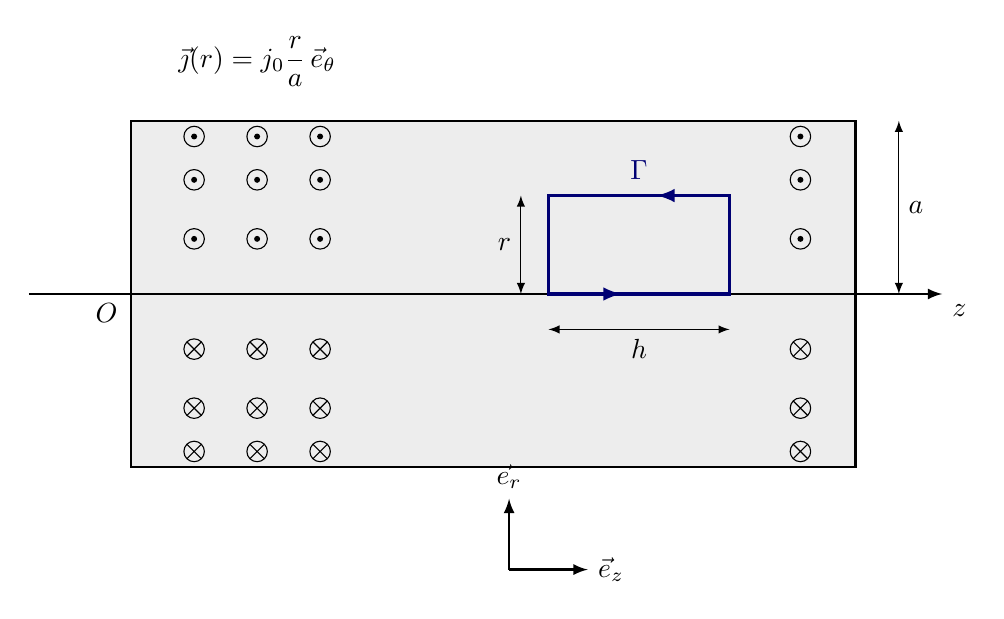
\begin{tikzpicture}[>=latex]
  \def\a{2.2}\def\rr{1.25}\def\zl{-4.8}\def\zr{4.4}\def\zz{0.5}\def\hh{2.3}

  % bobinage vu en coupe
  \fill[black!7] (\zl,-\a) rectangle (\zr,\a);
  \draw[thick] (\zl,-\a) rectangle (\zr,\a);

  % axe
  \draw[->,thick] (\zl-1.3,0) -- (\zr+1.1,0) node[below right]{$z$};
  \node[below left] at (\zl-0.05,0) {$O$};

  % courants orthoradiaux traversant le plan de figure
  \foreach \z in {-4.0,-3.2,-2.4} {
    \foreach \y in {0.7,1.45,2.0} { \sortant{\z}{\y} \entrant{\z}{-\y} }
  }
  \foreach \y in {0.7,1.45,2.0} { \sortant{3.7}{\y} \entrant{3.7}{-\y} }
  \node[align=center] at (-3.2,2.95) {$\vec{\jmath}(r)=j_0\dfrac{r}{a}\,\vec{e}_\theta$};

  % contour d'Ampere, oriente
  \draw[very thick, black!55!blue,
        postaction={decorate, decoration={markings,
          mark=at position 0.13 with {\arrow{latex}},
          mark=at position 0.63 with {\arrow{latex}}}}]
       (\zz,0) -- (\zz+\hh,0) -- (\zz+\hh,\rr) -- (\zz,\rr) -- cycle;
  \node[black!55!blue] at (\zz+\hh/2,\rr+0.32) {$\Gamma$};

  % cotes
  \draw[<->] (\zz,-0.45) -- (\zz+\hh,-0.45) node[midway,below]{$h$};
  \draw[<->] (\zz-0.35,0) -- (\zz-0.35,\rr) node[midway,left]{$r$};
  \draw[<->] (\zr+0.55,0) -- (\zr+0.55,\a) node[midway,right]{$a$};

  % base locale
  \draw[->,thick] (0,-3.5) -- (1.0,-3.5) node[right]{$\vec{e}_z$};
  \draw[->,thick] (0,-3.5) -- (0,-2.6) node[above]{$\vec{e}_r$};
\end{tikzpicture}
\end{document}
